\section{项目功能设计}

\subsection{总体功能说明}

\emph{大雾实验工具}是本组成员 2022 春季学期\textit{程序设计进阶与实践}的大作业项目。
本工具搭建于网页平台,支持任何设备自由访问。
传入实验数据后,本工具立刻完成绘制图像、计算不确定度、生成计算公式一系列操作,
并将最终结果整理成一份 \verb|Word| 文档,下载后即可直接使用。
本工具支持一级大物的所有实验(如表 \ref{tab:func}),大大提升了学生们撰写实验报告的效率。
由于本工具只是将传入的实验数据进行自动分析,故不会造成抄袭、造假等学术不端问题。

\subsection{具体功能点说明}

使用本工具时,用户只需输入他们做实验时测量到的原始数据,
而无需任何额外的计算处理,用户所要做的只有按照规定的格式上传 \verb|Excel| 文档。
本工具支持 \verb|xlsx|, \verb|csv| 等各种格式的数据表格。
具体而言,每个实验都会有一张示例数据表供用户参考,如图 \ref{fig:interface} 的界面所示。
用户也可以直接下载示例数据,并直接在它的基础上进行修改。
因此,本工具没有任何学习成本,是一款即点即用、免安装的简单轻应用。

\begin{figure}[htbp]
  \centering
  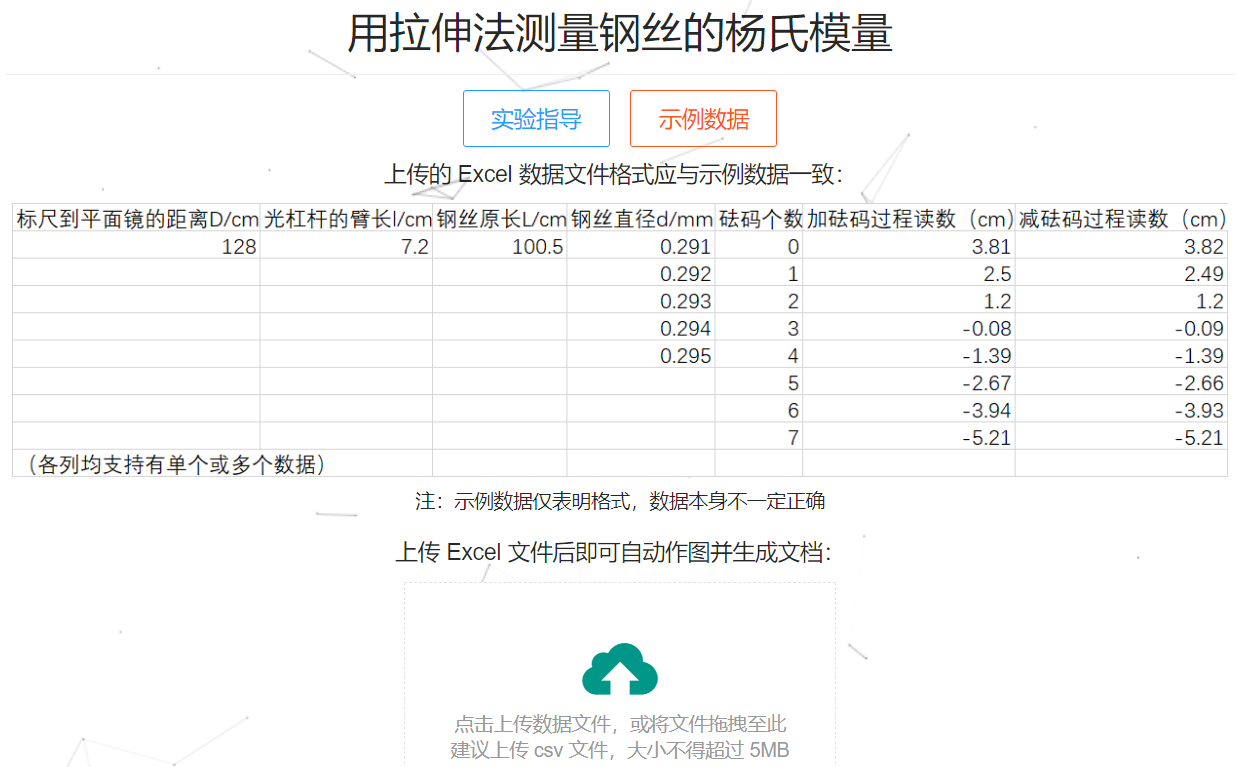
\includegraphics[width=\columnwidth]{figure/interface.png}
  \caption{“拉伸法测钢丝杨氏模量”的工具界面}
  \label{fig:interface}
\end{figure}

\subsubsection*{绘制图像}

本工具根据输入的数据以及实验原理,自动生成美观的实验图像。
本工具支持平滑去噪、数据拟合、双 y 图等多种图像生成需求,如图 \ref{fig:draw} 所示。

\begin{figure}[htbp]
  \centering
  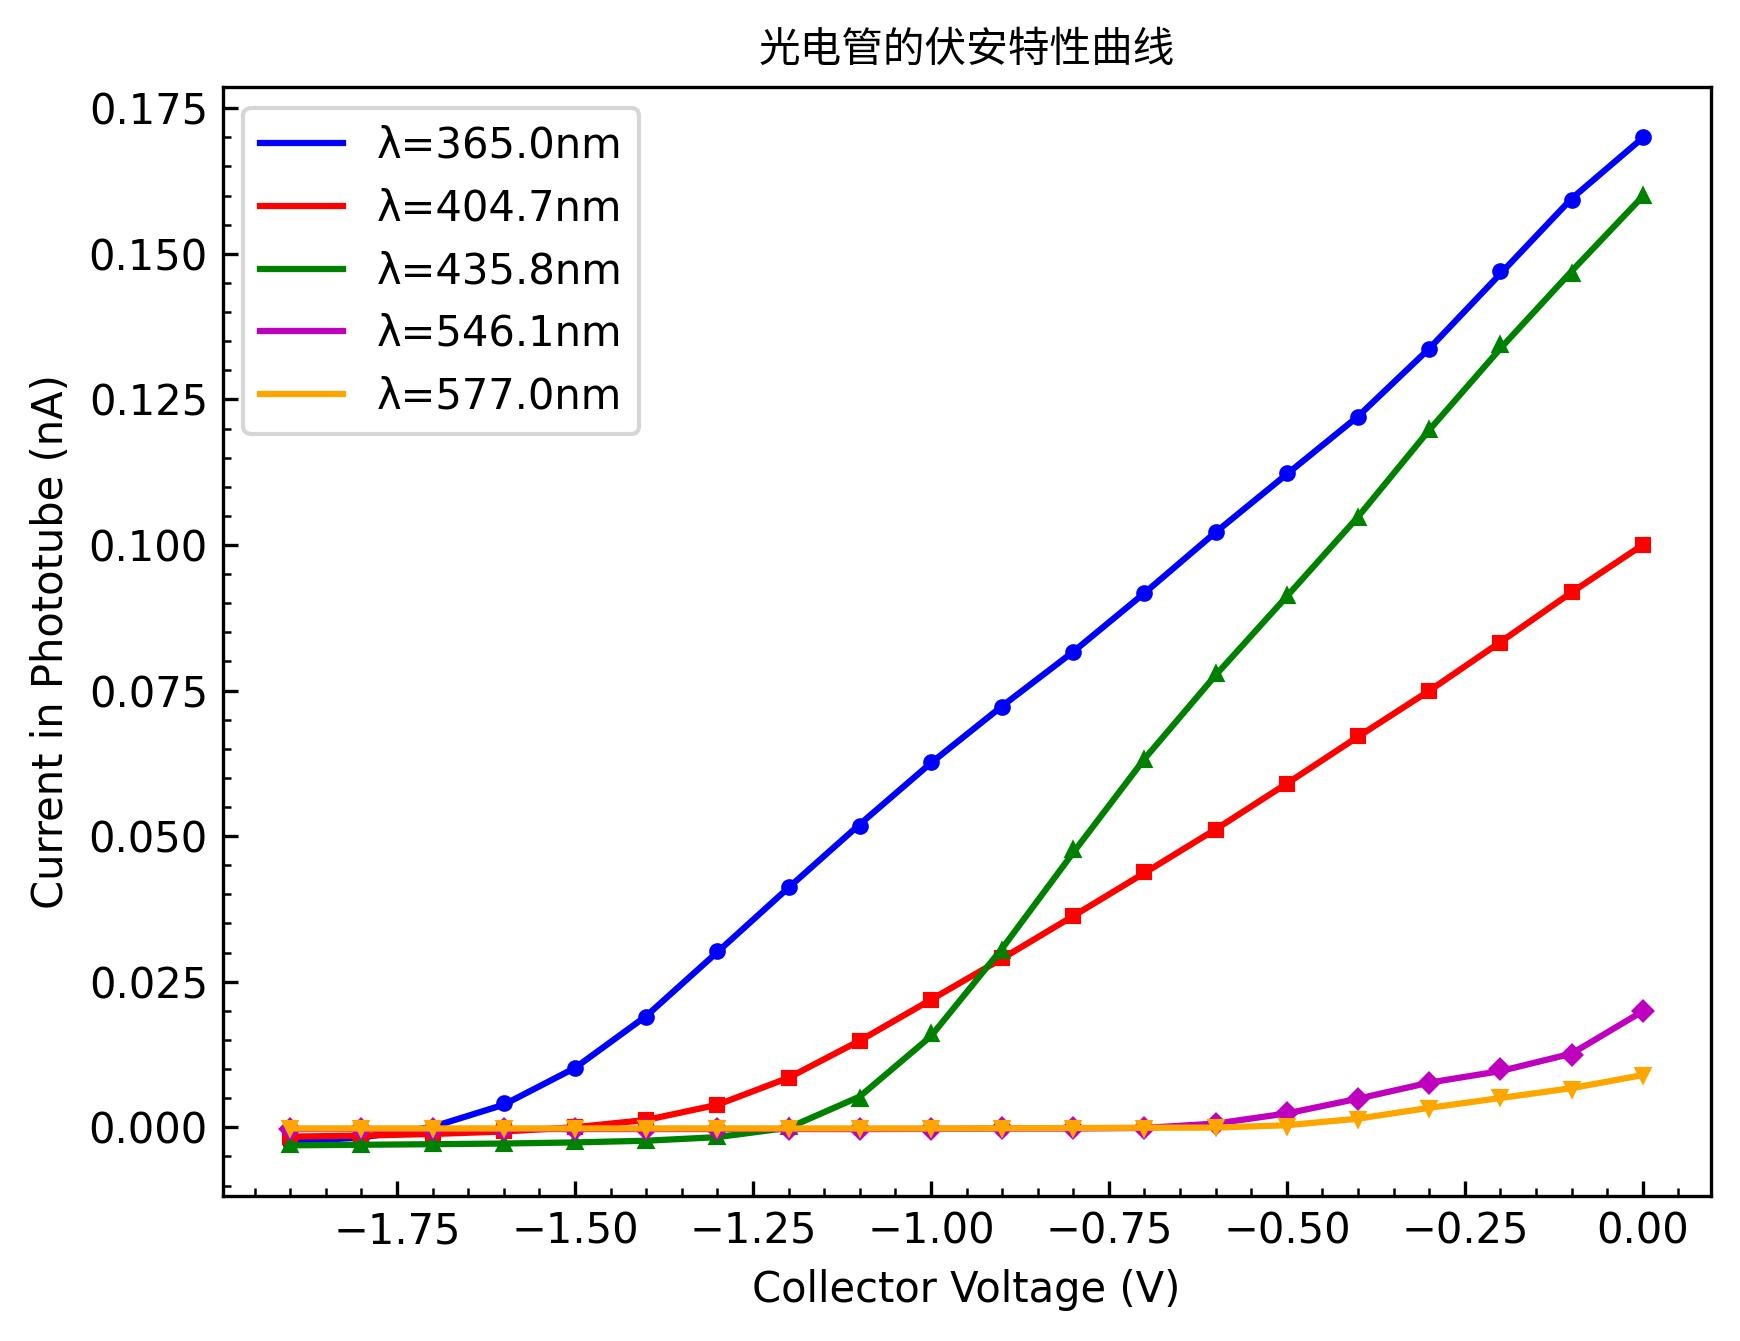
\includegraphics[width=\columnwidth]{figure/draw.jpg}
  \caption{平滑连接的光电效应伏安特性曲线}
  \label{fig:draw}
\end{figure}

\subsubsection*{计算不确定度}

本工具在生成的 \verb|Word| 文档中渲染了各种公式,如图 \ref{fig:calc} 所示。
用户可以直观看到不确定度每一步的计算过程,并在自己的报告中直接使用这些算式与结果。

\begin{figure}[htbp]
  \centering
  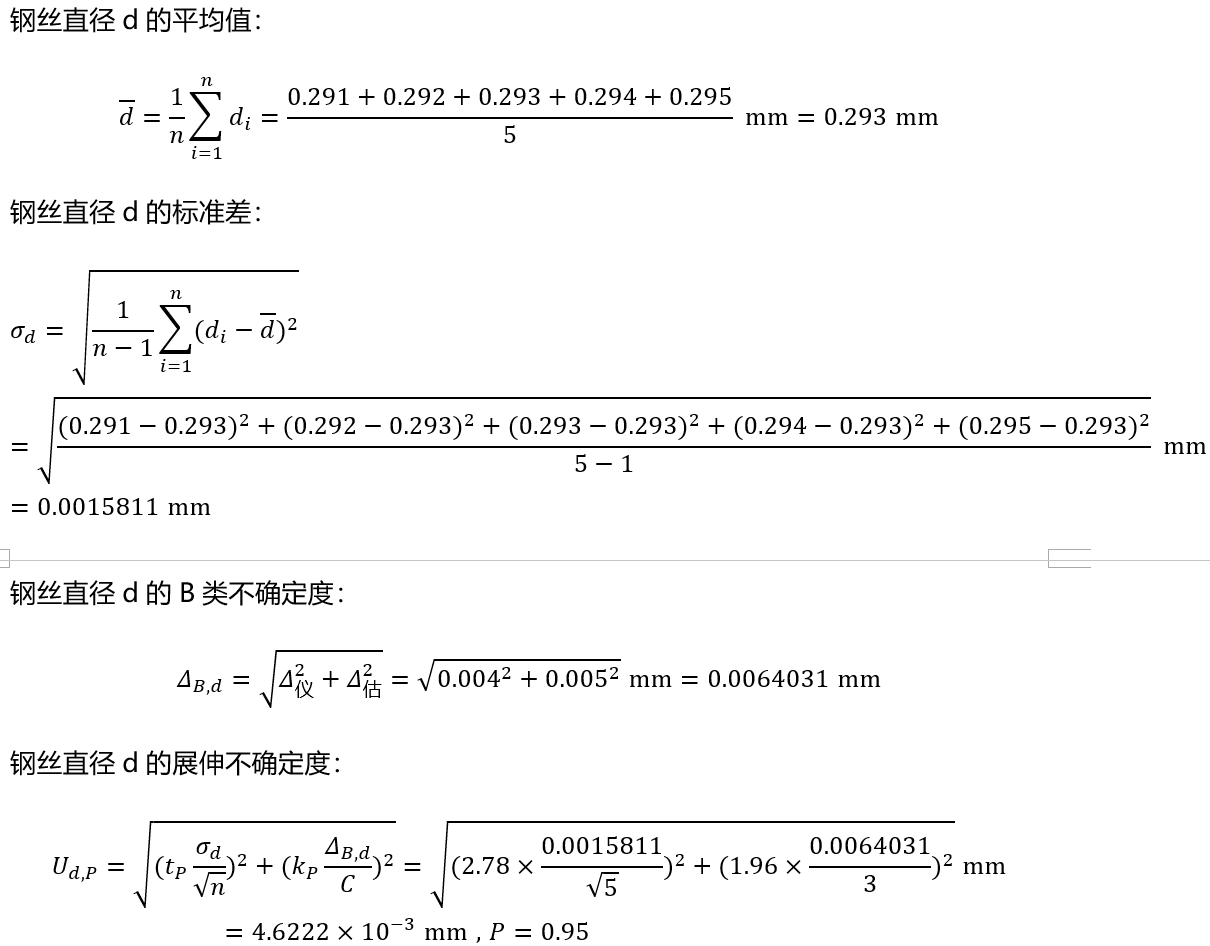
\includegraphics[width=\columnwidth]{figure/calc.png}
  \caption{不确定度计算的详细过程}
  \label{fig:calc}
\end{figure}

\subsubsection*{生成计算公式}

在 \verb|Word| 文档中除了有已经渲染好的公式外,
我们还提供了它们的\LaTeX源码,如图 \ref{fig:latex} 所示。
这极大方便了用\LaTeX, \verb|Markdown| 等排版实验报告的用户,他们再也不需要手动敲入每一个算式了。

\begin{figure}[htbp]
  \centering
  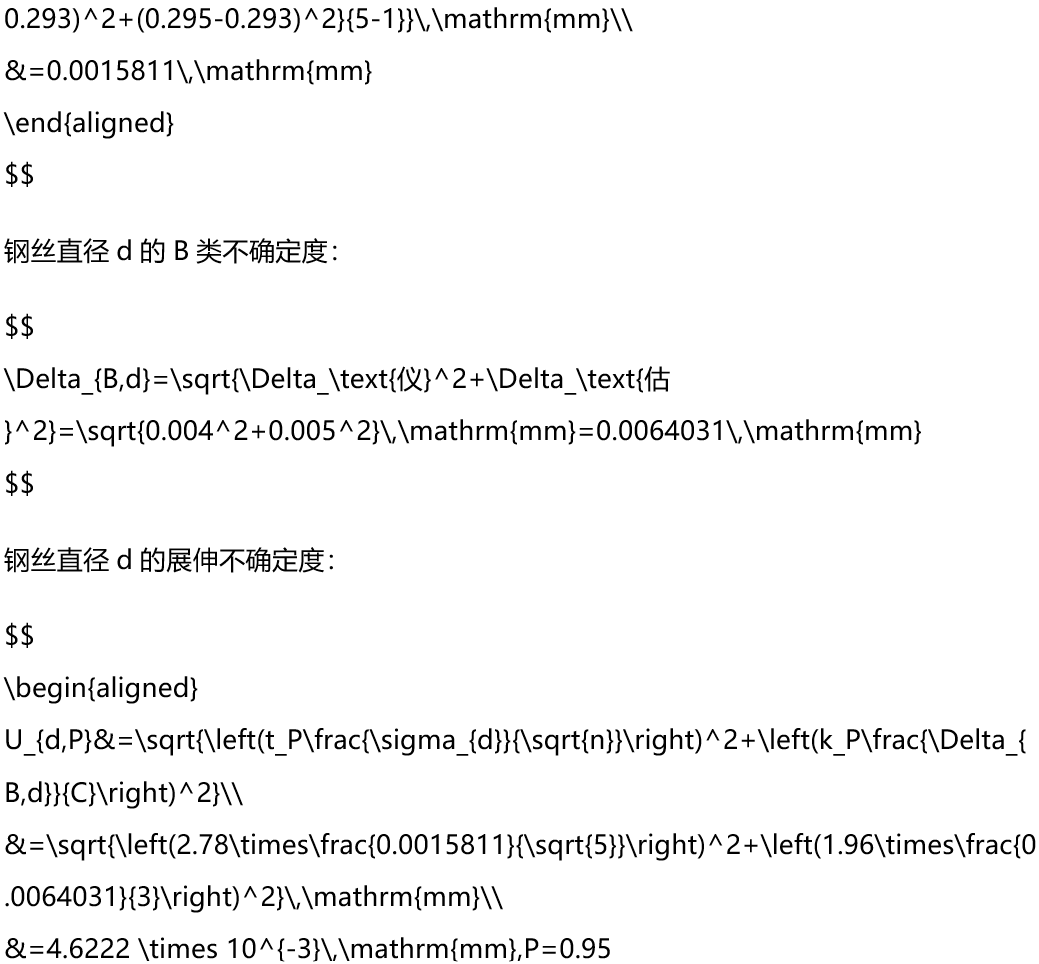
\includegraphics[width=\columnwidth]{figure/latex.png}
  \caption{不确定度算式的\LaTeX源码}
  \label{fig:latex}
\end{figure}

\subsection{功能点设计细节}

本工具后端使用 \verb|Python| 编写,使用的包与模块如表 \ref{tab:pkg} 所示。
前端由 \verb|HTML| 编写,并使用了 \verb|Flask| Web 应用框架。

\begin{table}[htbp]
  \caption{本工具使用的全部 \texttt{Python} 包与模块}
  \label{tab:pkg}
  \vskip 0.1in
  \centering\small
  \begin{tabular}{lc}
  \toprule
  \verb|Python| 包或模块 & 用途 \\
  \midrule
  \verb|chardet| & 检测用户上传的数据表格的编码 \\
  \verb|collections| & 通过 \verb|namedtuple| 使代码更清晰 \\
  \verb|Flask| & Web 应用框架 \\
  \verb|latex2mathml| & \LaTeX代码转换为 \verb|MathML| 代码 \\
  \verb|lxml| & 渲染 \verb|MathML| 代码以用于 \verb|Word| \\
  \verb|math|, \verb|numpy| & 不确定度数字运算 \\
  \verb|matplotlib| & 绘制物理图像 \\
  \verb|os|, \verb|random|, \verb|shutil| & 后台文件操作与管理 \\
  \verb|pandas| & 数据表格处理 \\
  \verb|python-docx| & 生成 \verb|Word| 文档 \\
  \verb|scipy| & 数据拟合 \\
  \verb|sympy| & 不确定度符号运算 \\
  \verb|time|, \verb|threading| & 定时删除生成的 \verb|Word| 文档 \\
  \verb|traceback| & 打印运行错误以便调试 \\
  \bottomrule
  \end{tabular}
  \vskip -0.1in
\end{table}

\subsubsection{图像绘制}

图像由 \verb|matplotlib| 绘制。我们的规范如下:

\begin{itemize}
  \item 面向绘图对象作图:\verb|fig, ax = matplotlib|\\\verb|.pyplot.subplots()|
  \item 设置副刻度为主刻度的一半,主刻度为默认:\verb|ax.xaxis.set_minor_locator(matplotlib|\\\verb|.ticker.AutoMinorLocator(2))|
  \item 刻度朝内:\verb|matplotlib.rcParams["xtick|\\\verb|.direction"] = matplotlib.rcParams|\\\verb|["ytick.direction"] = "in"|
  \item 若一张图有且只有一组点线,则点使用红色(\verb|color="r"|),线使用蓝色(\verb|color="b"|),且线覆盖在点的上面;若一张图有多组点线,则同一组点线的颜色应当相同,并依次使用蓝(\verb|b|)、红(\verb|r|)、绿(\verb|g|)、紫(\verb|m|)、橙(\verb|orange|)、青(\verb|c|)。
  \item 点的类型使用实心圆(\verb|"o"|),若一张图有多组点线,则依次使用实心圆(\verb|o|)、正方形(\verb|s|)、上三角(\verb|^|)、菱形(\verb|D|)、下三角(\verb|v|)、星号(\verb|*|)。
  \item 线条粗细使用 \verb|linewidth=1.5|, 点的大小使用 \verb|markersize=3|, 可视数据量、数据组数适当调整,但应保持统一性。
  \item 绘制双y轴图使用 \verb|twinx()| 方法。
  \item 只有一组点线的图,一般不显示图例。
  \item 图像字体:\verb|SourceHanSansSC-Regular.otf|
  \item 轴标签和标题中的物理量名称与单位应使用\LaTeX。
\end{itemize}

\subsubsection{数据处理}

无论使绘制图像时的线性拟合,还是计算不确定度的大小,都绕不开数据处理。
我们利用 \verb|pandas|, \verb|scipy|, \verb|sympy| 等包自主编写了 \verb|calc.py| 应用程序接口,
它提供以下函数:

\begin{description}
  \item[科学计数法输出] \verb|numlatex: (num: float,|\\\verb|prec: int = 5) -> str|\\
  \fbox{返回一个数的科学计数法形式的\LaTeX代码}\\
  \verb|num|: 要转成科学计数法的数字\\
  \verb|prec|: 有效数字位数(默认值:5)
  \item[不确定度计算] \verb|analyse: (data: pandas.DataFrame,|\\\verb|delta_b1: float = 0., delta_b2: float = 0.,|\\\verb|symbol: str = "x", unit: str = "",|\\\verb|confidence_C: float = 3., confidence_P:|\\\verb|float = 0.95) -> collections.namedtuple|\\\verb|("AnalyseData", ["average", "averagex",|\\\verb|"averagex2", "sigma", "sigmax", "sigmax2",|\\\verb|"delta_b", "delta_bx", "delta_bx2", "unc",|\\\verb|"uncx", "uncx2"])|\\
  \fbox{返回一组数据的平均值、标准差、不确定度}
  \verb|data|: 要处理的一组实验数据\\
  \verb|delta_b1|: 仪器最大允差 \(\Delta_\text{仪}\)(默认值:0)\\
  \verb|delta_b2|: 估读最大允差 \(\Delta_\text{估}\)(默认值:0)\\
  \verb|symbol|: 数据的物理符号(默认值:\verb|"x"|)\\
  \verb|unit|: 数据的单位(默认值:\verb|""|)\\
  \verb|confidence_C|: 置信系数 \(C\)(默认值:3)\\
  \verb|confidence_P|: 置信概率 \(P\)(缺省值:0.95)\\
  \verb|AnalyseData.average/averagex/averagex2|: 数据的平均值/平均值计算过程的\LaTeX代码/平均值计算过程的 \verb|MathML| 代码\\
  \verb|AnalyseData.sigma/sigmax/sigmax2|: 数据的标准差/标准差计算过程的\LaTeX代码/标准差计算过程的 \verb|MathML| 代码\\
  \verb|AnalyseData.delta_b/delta_bx/delta_bx2|: 数据的B类不确定度/B类不确定度计算过程的\LaTeX代码/B类不确定度计算过程的 \verb|MathML| 代码\\
  \verb|AnalyseData.unc/uncx/uncx2|: 数据的展伸不确定度/展伸不确定度计算过程的\LaTeX代码/展伸不确定度计算过程的 \verb|MathML| 代码
  \item[最小二乘法线性回归] \verb|analyse_lsm: (data_X:|\\\verb|pandas.DataFrame, data_Y: pandas|\\\verb|.DataFrame, symbol_X: str = "X",|\\\verb|symbol_Y: str = "Y", unit_m: str = "",|\\\verb|unit_b: str = "") -> collections|\\\verb|.namedtuple("AnalyseLsmData", ["m",|\\\verb|"mx", "mx2", "b", "bx", "bx2", "r",|\\\verb|"rx", "rx2", "s_m", "s_mx", "s_mx2",|\\\verb|"s_b", "s_bx", "s_bx2"])|\\
  \fbox{返回最小二乘法拟合数据得到的直线参数}\\
  \verb|data_X|: x轴数据(自变量数据)\\
  \verb|data_Y|: y轴数据(因变量数据)\\
  \verb|symbol_X|: 自变量物理符号(默认值:\verb|"X"|)\\
  \verb|symbol_Y|: 因变量物理符号(默认值:\verb|"Y"|)\\
  \verb|unit_m|: 斜率的单位(默认值:\verb|""|)\\
  \verb|unit_b|: 截距的单位(默认值:\verb|""|)\\
  \verb|AnalyseData.m/mx/mx2|: 拟合直线的斜率/斜率计算过程的\LaTeX代码/斜率计算过程的 \verb|MathML| 代码\\
  \verb|AnalyseData.b/bx/bx2|: 拟合直线的截距/截距计算过程的\LaTeX代码/截距计算过程的 \verb|MathML| 代码\\
  \verb|AnalyseData.r/rx/rx2|: 线性拟合的相关系数/相关系数计算过程的\LaTeX代码/相关系数计算过程的 \verb|MathML| 代码\\
  \verb|AnalyseData.s_m/s_mx/s_mx2|: 拟合直线的斜率标准差/斜率标准差计算过程的\LaTeX代码/斜率标准差计算过程的 \verb|MathML| 代码\\
  \verb|AnalyseData.s_b/s_bx/s_bx2|: 拟合直线的截距标准差/截距标准差计算过程的\LaTeX代码/截距标准差计算过程的 \verb|MathML| 代码
\end{description}